\subsubsection{Navier-Stokes方程式}
    \begin{align}
        \rho_\mathrm{f} (\partial _t + \boldsymbol{u} \cdot \boldsymbol{\nabla} ) \boldsymbol{u} &= 
            \boldsymbol{\nabla} \cdot \boldsymbol{\sigma} + 
            \rho_\mathrm{f} (\phi \boldsymbol{f}_\mathrm{p} + \boldsymbol{f}_\mathrm{sq} + \boldsymbol{f}_\mathrm{s}) \\
        \boldsymbol{\nabla} \cdot \boldsymbol{u} &= 0
    \end{align}

ここで,$t$は時間,
$\rho_\mathrm{f}$は流体の質量密度,
$\boldsymbol{\sigma}$は流体の応力テンソル,
$\phi \boldsymbol{f}_\mathrm{p}$は粒子の剛直性を保証する体積力,
$\boldsymbol{f}_\mathrm{sq}$は流体と粒子間の速度差を生じる力,
$\boldsymbol{f}_\mathrm{s}$はジグザグ流を生じる力である.
ジグザグ流とは,式\eqref{eq:zig_zag}のような速度プロファイルで表される流体の流れである.

    \begin{equation}
        v_x(y) =
        \begin{cases}
            \dot{\gamma} \left( - y -L_y/2 \right) & (-L_y/2 < y \geq -L_y/4) \\
            \dot{\gamma} y                        & (-L_y/4 < y \geq  L_y/4) \\
            \dot{\gamma} \left( - y + L_y/2 \right) & ( L_y/4 < y \geq  L_y/2)
        \end{cases}
        \label{eq:zig_zag}
    \end{equation}

    \begin{figure}[htbp]
        \centering
        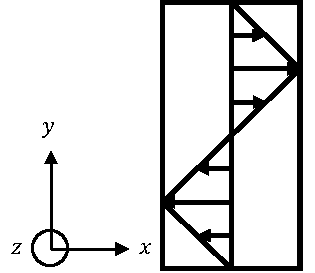
\includegraphics[scale=1.2]{/Users/taiga/Projects/lab/thesis/components/chapter2/figs/zig_zag.pdf}
        \caption{ジグザグ流の速度プロファイル}
        \label{fig:zig_zag}
    \end{figure}

\noindent
ここで,$\dot{\gamma}$はせん断速度,
$y$は$y$座標の値,
$L_y$は$y$軸方向の系の大きさである.
本研究では,せん断流を表現するためにジグザグ流を用いた.
